%%%%%%%%%%%%%%%%%%%%%%%%%%%%%%%%%%%%%%%%%%%%%%%%%%%%%%%%%%%%%%%%%%%%%%%%%%%%%%%
%% SOCIOL 723 -- Social Statistics II
%% Week 11 -- Synthetic Control and Its Extensions
%% Wenhao Jiang, Duke University, Fall 2026
%%%%%%%%%%%%%%%%%%%%%%%%%%%%%%%%%%%%%%%%%%%%%%%%%%%%%%%%%%%%%%%%%%%%%%%%%%%%%%%

\documentclass[aspectratio=169,11pt,xcolor=dvipsnames]{beamer}
\mode<presentation>

%% ---- fonts: Latin Modern Roman (the LaTeX default), serif throughout -------
\usepackage[T1]{fontenc}
\usepackage{lmodern}
\usefonttheme{serif}
\renewcommand{\familydefault}{\rmdefault}

%% ---- packages --------------------------------------------------------------
\usepackage{amsmath,amsfonts,amssymb,bm}
\usepackage{graphicx}
\usepackage{booktabs}
\usepackage{array}
\usepackage{tikz}
\usetikzlibrary{arrows.meta,positioning,calc}
\usepackage[english]{babel}

\newcommand{\srcp}[1]{{\scriptsize\color{gray}(#1)}}
\newcommand{\srct}[1]{#1}

\DeclareMathOperator*{\argminop}{arg\,min}
\DeclareMathOperator*{\argmaxop}{arg\,max}
%% \limits forces the subscript underneath even in inline math
\newcommand{\argmin}{\argminop\limits}
\newcommand{\argmax}{\argmaxop\limits}
\DeclareMathOperator{\Cov}{Cov}
\DeclareMathOperator{\Var}{Var}
\DeclareMathOperator{\trace}{tr}
\DeclareMathOperator{\rank}{rank}
\DeclareMathOperator{\plim}{plim}
\newcommand{\indep}{\perp\!\!\!\perp}

%% ---- notation conventions (course-wide) ------------------------------------
\newcommand{\E}{E}
\newcommand{\En}{\mathbb{E}_n}
\newcommand{\R}{\mathbb{R}}
\newcommand{\X}{\bm{X}}
\newcommand{\Y}{\bm{y}}
\newcommand{\Ix}{\bm{I}}
\newcommand{\zero}{\bm{0}}
\newcommand{\bhat}{\hat{\bm{\beta}}}
\newcommand{\dto}{\overset{d}{\longrightarrow}}
\newcommand{\pto}{\overset{p}{\longrightarrow}}
\usetikzlibrary{shapes,decorations.pathmorphing}
\newcommand{\lik}{\mathcal{L}}
\newcommand{\loglik}{\ell}
\newcommand{\Info}{\mathcal{I}}
\newcommand{\SE}{\mathrm{se}}

%% ---- theme -----------------------------------------------------------------
\usetheme{default}
%% thin single-line header: clickable section names, current one highlighted.
%% (miniframes is deliberately not used: one dot per slide wraps to 4 rows here)
\setbeamerfont{section in head/foot}{size=\tiny}
\setbeamertemplate{headline}{%
  \begin{beamercolorbox}[wd=\paperwidth,ht=2.4ex,dp=1.1ex,%
                         leftskip=.3cm,rightskip=.3cm]{section in head/foot}%
    \usebeamerfont{section in head/foot}%
    \insertsectionnavigationhorizontal{.94\paperwidth}{}{}%
  \end{beamercolorbox}%
}

\definecolor{dukeblue}{RGB}{1,33,105}
\definecolor{accent}{RGB}{200,78,0}
\definecolor{softgray}{RGB}{242,242,245}

\setbeamercolor{structure}{fg=dukeblue}
\setbeamercolor{frametitle}{fg=dukeblue,bg=white}
\setbeamercolor{section in head/foot}{fg=white,bg=dukeblue}
\setbeamercolor{section in head/foot shaded}{fg=white!50!dukeblue,bg=dukeblue}
\setbeamercolor{alerted text}{fg=accent}
\setbeamercolor{block title}{fg=white,bg=dukeblue}
\setbeamercolor{block body}{fg=black,bg=softgray}
\setbeamercolor{block title alerted}{fg=white,bg=accent}
\setbeamercolor{block body alerted}{fg=black,bg=softgray}

\setbeamertemplate{footline}[page number]
\setbeamertemplate{navigation symbols}{}
%% continued frames keep the SAME font size and spill onto a new slide
\setbeamertemplate{frametitle continuation}{\ifnum\insertcontinuationcount>1\normalfont\footnotesize\ (cont.)\fi}
\setbeamertemplate{itemize items}[circle]
\setbeamertemplate{blocks}[rounded][shadow=false]
\setbeamerfont{frametitle}{series=\bfseries}
\setbeamerfont{footnote}{size=\scriptsize}
\setbeamerfont{caption}{size=\footnotesize}
\setbeamertemplate{subsection in head/foot}{}
\setbeamertemplate{subsection in head/foot shaded}{}
\setbeamertemplate{caption}[numbered]

\newcommand{\adv}{\,\raisebox{0.6pt}{\textcolor{accent}{$\bigstar$}}}
%% marker for essential material every student must understand (examinable core)
\definecolor{corestar}{RGB}{0,83,155}
\newcommand{\core}{\,\raisebox{0.6pt}{\textcolor{corestar}{$\bigstar$}}}

\setbeamertemplate{section page}{%
  \begin{centering}\vfill
  {\usebeamercolor[fg]{structure}\Large\bfseries\insertsectionhead\par}
  \vskip4pt{\color{dukeblue}\rule{0.35\linewidth}{1pt}\par}
  \vfill\end{centering}}
\setbeamertemplate{subsection page}{%
  \begin{centering}\vfill
  {\usebeamercolor[fg]{structure}\large\bfseries\insertsubsectionhead\par}
  \vfill\end{centering}}

\AtBeginDocument{%
  \setlength{\abovedisplayskip}{5pt}%
  \setlength{\belowdisplayskip}{5pt}%
  \setlength{\abovedisplayshortskip}{2pt}%
  \setlength{\belowdisplayshortskip}{3pt}%
}
\setbeamertemplate{frametitle}{%
  \vskip4pt\usebeamerfont{frametitle}\usebeamercolor[fg]{frametitle}%
  \insertframetitle\par\vskip2pt}
\setbeamersize{text margin left=0.75cm, text margin right=0.75cm}

%% ---- title -----------------------------------------------------------------
%% ---- title page: same face as the body (Latin Modern), larger and bold
\setbeamerfont{title}{size*={16}{19},series=\bfseries}
\setbeamerfont{subtitle}{size=\Large,series=\mdseries}
\setbeamerfont{author}{size=\large}
\setbeamerfont{date}{size=\large}
\title[SOCIOL 723]{SOCIOL 723: Social Statistics II\\[-2pt]}
\subtitle{Week 11, Synthetic Control and Its Extensions\\[-6pt]}
\author[Jiang]{Wenhao Jiang\vspace{-2.5em}}
\institute[Duke]{}
\titlegraphic{
\includegraphics[height=1.3cm]{../Misc/duke_logo.png}}
\date{Department of Sociology, Fall 2026}


\begin{document}

\begin{frame}[plain]
  \titlepage
\end{frame}

\begin{frame}{Today}
  \tableofcontents
  \vskip6pt
  {\footnotesize \core{} $=$ essential, you must understand this \quad\quad \adv{} $=$ for understanding, not examined}
\end{frame}

\begin{frame}{When There Is Only One Treated Unit\core}
Difference-in-differences needs a control \emph{group}. What if the treated unit
is California, or East Germany, or a single firm?
\vskip4pt
\begin{itemize}\itemsep3pt
  \item Comparative case studies have always done this informally: ``compare
        California to the rest of the country.'' The choice of comparison was
        made by the author, and the reader had to trust it.
  \item \alert{Synthetic control} makes that choice a data-driven, transparent,
        pre-registered procedure: construct a weighted average of untreated units
        that reproduces the treated unit's pre-treatment trajectory.
  \item ``Arguably the most important innovation in the policy evaluation
        literature in the last 15 years'' \srcp{Athey and Imbens 2017}.
\end{itemize}
\vskip4pt
The identifying idea is not new. What is new is that the weights are chosen by an
algorithm, reported in a table, and checked against placebo units.
\end{frame}

\begin{frame}{Plan}
\textbf{Goal}: a counterfactual for one treated unit, how to judge it, and what
to do when the classic method does not fit.
\vskip3pt
\begin{enumerate}\itemsep2pt
  \item The estimator, its weights, and why the constraints matter; Proposition
        99 throughout, rebuilt from the data.
  \item What justifies it: a factor model, where bias comes from, and why the
        length of the pre-period does the work (a simulation).
  \item Inference with one treated unit: placebos, in-time placebos,
        leave-one-out, conformal tests, prediction intervals.
  \item Extensions: penalized and augmented SC, synthetic DiD, matrix completion
        and interactive fixed effects, many treated units.
  \item Applications: German reunification; Prop 47 and crime.
\end{enumerate}
\vskip3pt
{\footnotesize Data: \texttt{tidysynth::smoking}, 39 states 1970--2000; scripts
\texttt{figs/w11\_prop99.R}, \texttt{figs/w11\_sims.R}.}
\end{frame}


%%%%%%%%%%%%%%%%%%%%%%%%%%%%%%%%%%%%%%%%%%%%%%%%%%%%%%%%%%%%%%%%%%%%%%%%%%%%%%%
\section[Synthetic Control]{The Synthetic Control Estimator}
%%%%%%%%%%%%%%%%%%%%%%%%%%%%%%%%%%%%%%%%%%%%%%%%%%%%%%%%%%%%%%%%%%%%%%%%%%%%%%%
\begin{frame}\sectionpage\end{frame}

\begin{frame}{Setup\core}
Unit 1 is treated from period $T_0+1$ onward. Units $2,\dots,J+1$, the
\alert{donor pool}, are never treated. The estimand is
\begin{align*}
  \tau_{1t} = Y_{1t}(1) - Y_{1t}(0), \qquad t > T_0 .
\end{align*}
We observe $Y_{1t}(1)$; the whole problem is imputing $Y_{1t}(0)$.
\vskip4pt
\begin{block}{The synthetic control}
Choose weights $w_2,\dots,w_{J+1}$ with $w_j \geq 0$ and $\sum_j w_j = 1$ so that
the weighted donors match the treated unit \emph{before} treatment:
\begin{align*}
  \sum_{j\geq2} w_j Y_{jt} \approx Y_{1t} \ \text{ for } t \leq T_0,
  \qquad
  \sum_{j\geq2} w_j X_j \approx X_1 ,
\end{align*}
then estimate $\hat\tau_{1t} = Y_{1t} - \sum_{j\geq2} w_j Y_{jt}$ for $t > T_0$.
\end{block}
\end{frame}

\begin{frame}{Running Example: Proposition 99}
California raised its cigarette tax by 25 cents a pack in 1989 and funded
anti-smoking campaigns. Outcome: packs sold per capita. Donors: 38 states with
no large tobacco program or tax increase in the period.
\vskip-2pt
\begin{center}
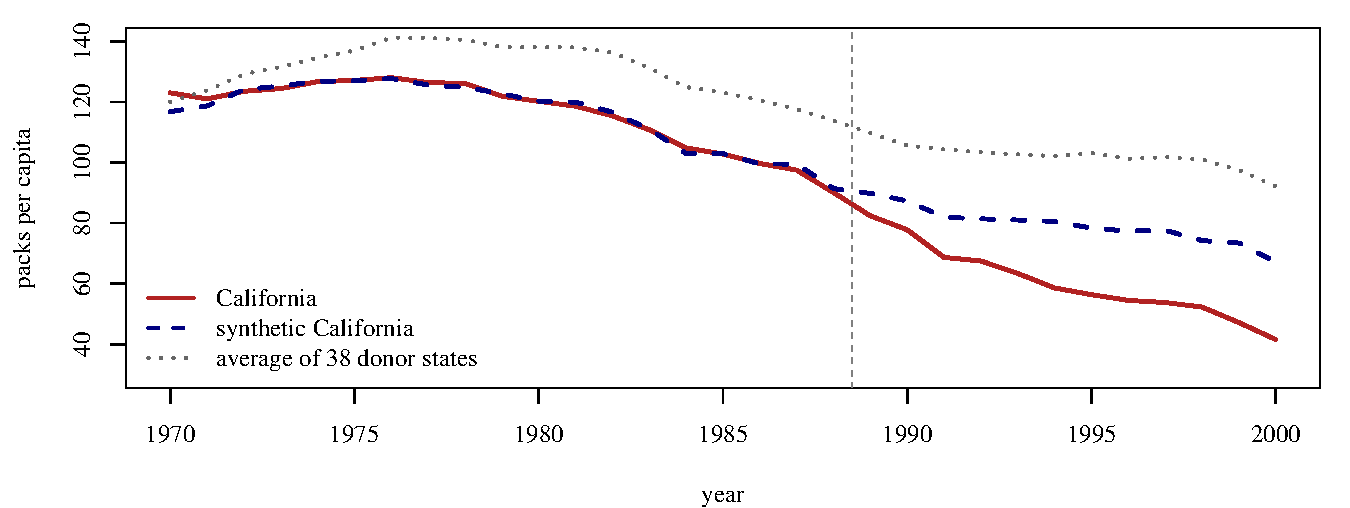
\includegraphics[width=0.72\linewidth]{figs/prop99_paths.pdf}
\end{center}
\vskip-9pt
\begin{itemize}\itemsep1pt
  \item The donor average is a poor counterfactual: California was already
        falling faster before 1989 (1988: 90.1 against 113.8).
  \item The synthetic California tracks it to 1988 and then separates
        \srcp{figs/w11\_prop99.R}.
\end{itemize}
\end{frame}



\begin{frame}{The Optimization Problem, Explicitly\adv}
Let $\bm X_1$ be a $k\times1$ vector of pre-treatment predictors for the treated
unit and $\bm X_0$ the $k\times J$ matrix for the donors. Choose weights
\begin{align*}
  \bm W^{*}(\bm V) = \argmin_{\bm W \in \mathcal{W}}\ (\bm X_1 - \bm X_0\bm W)'\,
  \bm V\,(\bm X_1 - \bm X_0 \bm W) ,
  \qquad
  \mathcal W = \Big\{\bm W \geq 0,\ \textstyle\sum_j w_j = 1\Big\} .
\end{align*}
\vskip3pt
\begin{itemize}\itemsep3pt
  \item $\bm V$ is a diagonal matrix of \alert{predictor importance} weights. It
        is itself chosen, usually to minimize pre-treatment prediction error
        of the \emph{outcome}:
        $\bm V^{*} = \argmin_{\bm V} \sum_{t\leq T_0}\big(Y_{1t} - \sum_j w_j^{*}(\bm V) Y_{jt}\big)^2$.
  \item So there are two nested optimizations, and the inner one is a constrained
        quadratic program. The constraint set $\mathcal W$ is a simplex.
  \item \alert{This nesting is where researcher degrees of freedom hide.} Which
        predictors enter $\bm X$, and how many pre-periods are used, can move the
        answer. Pre-register the choice or report the full space.
\end{itemize}
\end{frame}

\begin{frame}{The Weights and the Balance on Prop 99}
Predictors as in \srct{Abadie, Diamond, and Hainmueller (2010)}: income, price,
share aged 15--24 (1980--88), beer (1984--88), sales in 1975, 1980, 1988.
\begin{columns}[T]
\begin{column}{0.4\linewidth}
\begin{center}\footnotesize
\renewcommand{\arraystretch}{1.1}
\begin{tabular}{@{}lcc@{}}
\toprule
state & ours & ADH \\
\midrule
Utah & 0.342 & 0.334 \\
Nevada & 0.238 & 0.234 \\
Montana & 0.209 & 0.199 \\
Colorado & 0.149 & 0.164 \\
Connecticut & 0.062 & 0.069 \\
other 33 & 0 & 0 \\
\bottomrule
\end{tabular}
\end{center}
\end{column}
\begin{column}{0.56\linewidth}
\begin{center}\footnotesize
\renewcommand{\arraystretch}{1.1}
\begin{tabular}{@{}lccc@{}}
\toprule
predictor & CA & synth. & donors \\
\midrule
log income & 10.08 & 9.85 & 9.83 \\
retail price & 89.4 & 89.4 & 87.3 \\
share 15--24 & .174 & .174 & .173 \\
beer & 24.3 & 24.2 & 23.7 \\
sales 1975 & 127.1 & 127.0 & 136.9 \\
sales 1980 & 120.2 & 120.2 & 138.1 \\
sales 1988 & 90.1 & 91.4 & 113.8 \\
\bottomrule
\end{tabular}
\end{center}
\end{column}
\end{columns}
\vskip2pt
\begin{itemize}\itemsep0pt
  \item Five states carry all the weight. Pre-period RMSPE 1.78 packs.
  \item Average gap 1989--2000: $-18.8$ packs (about $-24\%$); in 2000: $-25.6$.
  \item Income is not matched: California is richer than any combination.
\end{itemize}
\end{frame}


\begin{frame}[allowframebreaks,t]{The Factor-Model Justification\adv}
Matching California's \emph{past} is only useful if it tells us something about
California's missing \emph{future}. Why should it? The factor model is the answer:
it states the conditions under which a good pre-treatment fit licenses that
extrapolation.
\vskip3pt
Suppose untreated outcomes follow a linear factor model
\begin{align*}
  Y_{jt}(0) = \delta_t + \bm\theta_t'\bm Z_j + \bm\lambda_t'\bm\mu_j + \epsilon_{jt} ,
\end{align*}
with $\bm\lambda_t$ common (unobserved) factors and $\bm\mu_j$ unit-specific
loadings.
\vskip3pt
\begin{itemize}\itemsep3pt
  \item \textbf{DID} allows arbitrary common time shocks $\delta_t$, but requires
        that the remaining term $\bm\lambda_t'\bm\mu_j$ not generate
        \emph{differential} trends between treated and control units. Synthetic
        control weakens that by matching on the loadings instead.
  \item \srct{Abadie, Diamond, and Hainmueller (2010)} show that if a convex
        combination of donors reproduces the treated unit's outcomes over a
        \emph{long} pre-period \emph{and} its observed predictors, then under
        regularity conditions, enough pre-periods relative to the noise, and a
        factor structure of bounded rank, the weighted donors also approximately
        match the \alert{unobserved loadings} $\bm\mu_1$, and a bound on the
        post-treatment bias shrinks with the number of pre-periods.
  \item \alert{Length of the pre-period is doing the identification work.} A
        two-period match proves nothing; a twenty-period match is informative.
        This is the single most important design consideration.
\end{itemize}
\end{frame}

\begin{frame}{Where the Bias Comes From}
Write the factor model for treated and synthetic units after treatment ($t > T_0$):
\begin{align*}
  Y_{1t}(0) - \textstyle\sum_j w_j Y_{jt}(0)
  &= \bm\theta_t'\big(\bm Z_1 - \textstyle\sum_j w_j\bm Z_j\big)
   + \bm\lambda_t'\big(\bm\mu_1 - \textstyle\sum_j w_j\bm\mu_j\big) \\
  &\quad + \big(\epsilon_{1t} - \textstyle\sum_j w_j\epsilon_{jt}\big)
   \qquad \text{\footnotesize $\delta_t$ cancels: $\textstyle\sum_j w_j = 1$}
\end{align*}
\begin{itemize}\itemsep2pt
  \item A good pre-period fit matches $\bm Z$ and, over many periods, can only be
        achieved by matching the loadings $\bm\mu_1$: the middle term is small.
  \item With few pre-periods, the weights can instead \alert{fit the noise}
        $\epsilon_{1t}$: a tight fit that says nothing about $\bm\mu$.
  \item The bound in \srct{Abadie, Diamond, and Hainmueller (2010)} falls with
        $T_0$ only if the fit is good, and rises with the number of donors $J$:
        more donors make it easier to fit noise \srcp{Abadie 2021}.
  \item DiD is the case $w_j = 1/J$ plus a level shift: unbiased only if
        $\bm\mu_1$ equals the donors' average loading.
\end{itemize}
\end{frame}

\begin{frame}{Simulation: the Pre-Period Does the Work}
Two factors, 20 donors, the treated unit's loadings inside the donors' hull but
far from their average; true effect 0; 1,000 draws \srcp{figs/w11\_sims.R}.
\vskip3pt
\begin{center}\footnotesize
\renewcommand{\arraystretch}{1.0}
\begin{tabular}{@{}lccccc@{}}
\toprule
pre-periods $T_0$ & 3 & 5 & 10 & 20 & 40 \\
\midrule
\multicolumn{6}{@{}l}{\emph{low noise} ($\sigma = 0.25$): root mean squared error} \\
synthetic control & 0.44 & 0.38 & 0.27 & 0.19 & 0.14 \\
difference-in-differences & 0.39 & 0.40 & 0.39 & 0.43 & 0.49 \\
\midrule
\multicolumn{6}{@{}l}{\emph{high noise} ($\sigma = 1$)} \\
synthetic control & 0.68 & 0.67 & 0.66 & 0.56 & 0.47 \\
difference-in-differences & 0.78 & 0.67 & 0.60 & 0.55 & 0.56 \\
SC pre-period RMSPE & 0.22 & 0.38 & 0.63 & 0.79 & 0.90 \\
\bottomrule
\end{tabular}
\end{center}
\vskip3pt
\begin{itemize}\itemsep2pt
  \item With little noise, SC improves steadily with $T_0$; DiD's bias does not shrink.
  \item With much noise and short $T_0$, SC is no better than DiD, and its
        pre-period fit (0.22) is \alert{tighter than the noise} ($\sigma = 1$): it fit
        the noise. A suspiciously perfect fit is a warning, not a reassurance.
\end{itemize}
\end{frame}


\begin{frame}{Why the Constraints Matter\core}
The restrictions $w_j\geq 0$ and $\sum_j w_j = 1$ look like technicalities. They
are the heart of the method.
\vskip4pt
\begin{itemize}\itemsep3pt
  \item \textbf{No extrapolation}: the synthetic unit is a \emph{convex
        combination} of real units, so it lies inside the donor pool's support.
        Unconstrained regression would happily assign weights of $+3$ and $-2$ and
        predict outside anything ever observed.
  \item \textbf{Sparsity}: the constraints usually produce weights on a handful
        of donors and zero on the rest. You can print the weight table and let
        readers judge whether the comparison is sensible.
  \item \textbf{Transparency}: the counterfactual is a named, weighted set of real
        places, not a regression coefficient.
  \item If no convex combination matches the treated unit, if California is
        richer than every donor, \alert{the method tells you}, through poor
        pre-treatment fit. That is a feature.
\end{itemize}
\end{frame}

\begin{frame}{What the Constraints Prevent, on Prop 99}
Drop $w_j \geq 0$ and keep $\sum_j w_j = 1$: with 38 donors and 19 pre-years,
infinitely many weightings fit the pre-period exactly. Take the smallest one
(minimum norm) \srcp{figs/w11\_prop99.R}:
\vskip4pt
\begin{center}\small
\renewcommand{\arraystretch}{1.12}
\begin{tabular}{@{}lcc@{}}
\toprule
 & SC weights & regression weights \\
\midrule
nonzero donors & 5 & 38 \\
negative weights & 0 & 17 (as low as $-0.13$, Tennessee) \\
pre-period fit & RMSPE 1.78 & exact \\
average gap 1989--2000 & $-18.8$ & $-15.5$ \\
\bottomrule
\end{tabular}
\end{center}
\vskip4pt
\begin{itemize}\itemsep2pt
  \item An exact fit with $J > T_0$ is guaranteed and therefore uninformative: it
        fits the noise.
  \item Negative weights mean the counterfactual California is ``West Virginia
        plus Connecticut minus Tennessee minus Mississippi'': extrapolation no
        reader can inspect \srcp{Abadie 2021}.
\end{itemize}
\end{frame}



\begin{frame}{Relation to Difference-in-Differences\core}
DID is synthetic control with the weights fixed at $1/J$ (or population shares),
and with an added intercept shift.
\vskip4pt
\begin{itemize}\itemsep3pt
  \item DID assumes parallel trends between the treated unit and a
        \emph{pre-specified} average of controls.
  \item Synthetic control \emph{searches} for a weighting under which
        pre-treatment trajectories coincide, and then assumes that coincidence
        continues. The factor model on the previous frame states when that
        assumption is warranted.
  \item So the two methods sit on a spectrum: DID trusts a pre-specified
        comparison and an intercept shift; synthetic control trusts a fitted
        comparison and no intercept. Synthetic DID (later today) combines them.
\end{itemize}
\end{frame}

\begin{frame}[allowframebreaks,t]{Inference With One Treated Unit\core}
Conventional standard errors are meaningless here: $n_{\text{treated}} = 1$, and
the usual asymptotics run in the number of treated units. Instead,
\alert{permutation inference}.
\vskip3pt
\begin{block}{Placebo (in-space) tests}
Pretend each donor was the treated unit and estimate its ``effect.'' If the real
treated unit's post-treatment gap is extreme relative to the placebo
distribution, that is evidence.
\end{block}
\vskip3pt
For each unit $j$ compute
\begin{align*}
  \text{RMSPE}^{\text{pre}}_j = \sqrt{\tfrac{1}{T_0}\sum_{t\leq T_0}\big(Y_{jt}-\hat Y^{N}_{jt}\big)^2},
  \qquad
  \text{RMSPE}^{\text{post}}_j = \sqrt{\tfrac{1}{T-T_0}\sum_{t> T_0}\big(Y_{jt}-\hat Y^{N}_{jt}\big)^2},
\end{align*}
and rank units by the \alert{ratio} $\text{RMSPE}^{\text{post}}_j /
\text{RMSPE}^{\text{pre}}_j$.
\vskip3pt
\begin{itemize}\itemsep2pt
  \item The ratio, rather than the raw post-treatment gap, is what makes placebos
        comparable: a donor the method could not fit will show a large gap for
        reasons unrelated to treatment. \textbf{Discard poorly fitting placebos.}
  \item The rank of the treated unit among the $J+1$ units gives a
        permutation-style $p$-value: with 38 donors the smallest attainable value
        is $1/39 \approx 0.026$. \alert{Call it a placebo rank, not an exact
        $p$-value}: exactness would require treatment to have been randomly
        assigned among these units under a sharp null, which it was not.
  \item \textbf{In-time placebo}: re-run pretending treatment began earlier. A gap
        should not appear before the real intervention.
  \item \textbf{Leave-one-donor-out}: drop each positively weighted donor in turn.
        If the result rests on one unit, say so.
\end{itemize}
\end{frame}

\begin{frame}{Placebos on Prop 99}
\vskip-2pt
\begin{center}
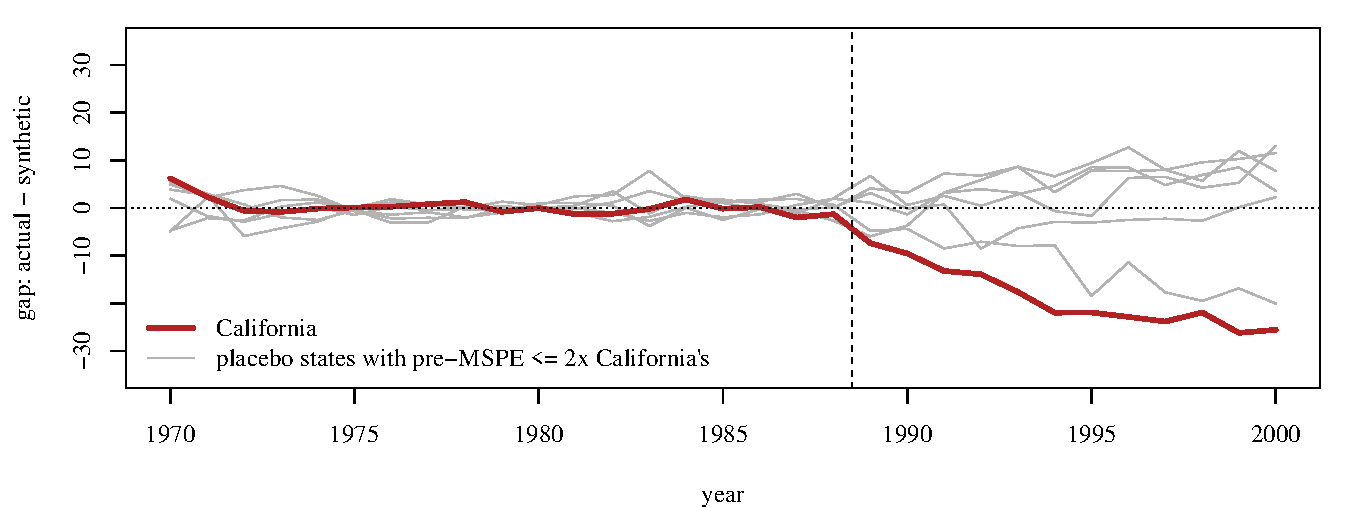
\includegraphics[width=0.8\linewidth]{figs/prop99_placebos.pdf}
\end{center}
\vskip-9pt
\begin{itemize}\itemsep1pt\small
  \item Pre-period MSPE: California 3.17; median donor 15.4. Only 6 donors fit
        as well as twice California's MSPE (shown).
  \item Post/pre MSPE ratio: California 124, largest of 39 (next: Georgia, 47).
        Placebo rank $1/39 = 0.026$, the smallest attainable.
\end{itemize}
\end{frame}

\begin{frame}{In-Time Placebo and Leave-One-Out on Prop 99}
Outcome-only weights (all 19 pre-years) give nearly the same answer: average
gap $-19.5$, pre-RMSPE 1.66 \srcp{figs/w11\_prop99.R}.
\vskip4pt
\textbf{In-time placebo}: pretend the law came in 1980, fit on 1970--79.
\begin{itemize}\itemsep1pt
  \item Fit 1970--79: RMSPE 0.84. Average gap 1980--88: $-3.4$ packs.
  \item Not zero: California was already pulling away in the 1980s, by about
        a sixth of the post-1989 effect. Report it.
\end{itemize}
\vskip4pt
\textbf{Leave-one-out}: drop each donor with positive weight, refit.
\begin{center}\small
\renewcommand{\arraystretch}{1.1}
\begin{tabular}{@{}lcccccc@{}}
\toprule
dropped & Utah & Montana & Nevada & Connecticut & N.\ Hampshire & Colorado \\
\midrule
average gap & $-19.1$ & $-18.0$ & $-19.2$ & $-20.5$ & $-19.8$ & $-19.6$ \\
\bottomrule
\end{tabular}
\end{center}
\vskip2pt
No single donor drives the estimate.
\end{frame}

\begin{frame}{Conformal Inference \srcp{Chernozhukov, Wüthrich, and Zhu 2021}}
Placebos permute \emph{units}. Conformal inference permutes \emph{time}, for one
hypothesis at a time.
\vskip2pt
\begin{enumerate}\itemsep2pt
  \item Hypothesis $H_0$: $\tau_t = \tau_t^0$ for $t > T_0$ (start with $\tau^0 = 0$).
        Under $H_0$, $Y_{1t} - \tau_t^0$ is the untreated outcome in every period.
  \item Fit the weights on \emph{all} $T$ periods using that series; residuals $\hat u_t$.
  \item Statistic $S = $ mean $|\hat u_t|$ over post-periods. Recompute it for every
        cyclic shift of the residuals in time; the $p$-value is the share at least
        as large.
  \item Invert: the set of $\tau^0$ not rejected is a confidence set.
\end{enumerate}
\vskip3pt
\begin{itemize}\itemsep2pt
  \item Valid when residuals are exchangeable (or weakly dependent) over time.
  \item Prop 99, $H_0$: no effect in any year: $S = 13.5$, $p = 0.097$ with 31
        shifts. Weaker evidence than the placebo rank: here the null is
        tested against the state's own residual noise.
\end{itemize}
{\footnotesize Prediction intervals that combine weight-estimation and post-period
uncertainty: \srct{Cattaneo, Feng, and Titiunik (2021)}, \texttt{scpi}.}
\end{frame}


\begin{frame}[allowframebreaks,t]{The Canonical Application: California Proposition 99}
\srct{Abadie, Diamond, and Hainmueller (2010)} study California's 1988 tobacco
control programme.
\vskip3pt
\begin{itemize}\itemsep3pt
  \item \textbf{Outcome}: per-capita cigarette sales, 1970--2000.
        \textbf{Donor pool}: the 38 states that never adopted comparable
        programmes over the period, states with their own large tax increases
        or programmes are excluded \emph{a priori}, on substantive grounds.
  \item \textbf{Synthetic California} is a weighted average of Colorado,
        Connecticut, Montana, Nevada, and Utah. The weight table is printed in the
        paper, and readers can judge whether that is a sensible California.
  \item Pre-1988 trajectories are nearly indistinguishable; afterwards they
        diverge sharply, implying roughly 26 fewer packs per capita per year by
        2000.
  \item In the placebo distribution, California's post/pre RMSPE ratio is the
        largest of all 39 units, giving $p = 1/39$.
\end{itemize}
\vskip2pt
\alert{Notice how much of the credibility comes from things a reader can check by
eye}: the weight table, the pre-treatment overlap, and the placebo plot.
\end{frame}

\begin{frame}{In the Literature: German Reunification}
\vskip-2pt{\footnotesize\color{gray}\srct{Abadie, Diamond, and Hainmueller (2015)}}\vskip1pt
\textbf{The question}: what did reunification in 1990 cost West Germany?
GDP per capita (PPP, 2002 USD); 16 OECD donors; predictors trained on
1971--80, validated on 1981--90.
\begin{columns}[T]
\begin{column}{0.44\linewidth}
\begin{center}\footnotesize
\renewcommand{\arraystretch}{1.0}
\begin{tabular}{@{}lc@{}}
\toprule
donor & weight \\
\midrule
Austria & 0.42 \\
United States & 0.22 \\
Japan & 0.16 \\
Switzerland & 0.11 \\
Netherlands & 0.09 \\
\bottomrule
\end{tabular}
\end{center}
{\scriptsize Regression weights: Greece $-0.09$, Portugal $-0.08$, Italy $-0.05$.}
\end{column}
\begin{column}{0.54\linewidth}
\footnotesize
\begin{itemize}\itemsep1pt
  \item About $-1{,}600$ USD per person per year, 1990--2003; 2003 GDP per capita
        12\% below synthetic.
  \item In-time placebo, reunification in 1975: no gap.
  \item Post/pre RMSPE ratio about 16, largest of 17: $p = 1/17 \approx 0.06$.
  \item Leave-one-out: dropping the US gives the smallest effect, about $-630$
        USD per year.
\end{itemize}
\end{column}
\end{columns}
\vskip3pt
{\footnotesize Replications across software packages and variable orderings do not
reproduce the published weights \srcp{Klößner et al.\ 2018}: $\bm V$ is poorly identified.}
\end{frame}



\begin{frame}{Diagnostics and Failure Modes\core}
\begin{itemize}\itemsep3pt
  \item \textbf{Poor pre-treatment fit} invalidates the design. Report the
        pre-treatment RMSPE and plot the two trajectories. If they do not overlap
        before treatment, stop.
  \item \textbf{Interpolation bias}: donors very unlike the treated unit can be
        combined to match on average while differing on everything that matters.
        Restrict the donor pool on substantive grounds \emph{before} estimating.
  \item \textbf{Overfitting the pre-period}: matching noise rather than structure.
        A long pre-period and few donors is the safe configuration.
  \item \textbf{Contamination}: donors affected by the treatment (spillovers) or
        by their own interventions must be excluded.
  \item \textbf{Specification search}: the choice of predictors and pre-periods
        can move results. Pre-register it, or report the full space.
\end{itemize}
\end{frame}

\begin{frame}{Covariates or Lagged Outcomes?}
\begin{itemize}\itemsep4pt
  \item If \emph{every} pre-period outcome enters $\bm X_1$ separately, the
        optimal $\bm V$ puts all its weight on them and the covariates become
        irrelevant, however predictive \srcp{Kaul, Klößner, Pfeifer, and Schieler 2022}.
  \item Prop 99 illustrates both choices: ADH predictors give $-18.8$;
        all 19 pre-period outcomes alone give $-19.5$.
  \item Matching on covariates protects against fitting noise in the outcome
        path; matching on outcomes protects against unmeasured loadings. Report
        both when they differ.
  \item $\bm V$ is chosen by a nested, non-convex optimization; different software
        returns different $\bm V$ and weights for the same data
        \srcp{Klößner et al.\ 2018}. Report the weights, not only the gap.
\end{itemize}
\end{frame}

\begin{frame}{The Basque Country: Two Good Fits, Two Answers}
\srct{Abadie and Gardeazabal (2003)}: GDP per capita in the Basque Country after
terrorism began around 1970; 16 other Spanish regions as donors
\srcp{\texttt{Synth::basque}; figs/w11\_more.R}.
\begin{center}\small
\renewcommand{\arraystretch}{1.12}
\begin{tabular}{@{}l>{\raggedright\arraybackslash}p{3.6cm}>{\raggedright\arraybackslash}p{3.9cm}@{}}
\toprule
 & predictors (Synth example) & pre-period outcomes only \\
\midrule
weights & Catalu\~na 0.851, Madrid 0.149 & Madrid 0.483, Baleares 0.311, Rioja 0.206 \\
pre-period RMSPE & 0.094 & 0.076 \\
gap 1975--97 (thousand 1986 USD) & $-0.70$ & $-1.04$ \ ($-11.5\%$) \\
\bottomrule
\end{tabular}
\end{center}
\vskip2pt
\begin{itemize}\itemsep1pt
  \item Both fit the pre-period almost perfectly, with \emph{disjoint} donors
        except Madrid. The weights are not unique when several combinations
        track the treated unit \srcp{Abadie 2021}.
  \item The sign is robust; the size depends on the specification. Report the
        specifications you tried.
\end{itemize}
\end{frame}



%%%%%%%%%%%%%%%%%%%%%%%%%%%%%%%%%%%%%%%%%%%%%%%%%%%%%%%%%%%%%%%%%%%%%%%%%%%%%%%
\section[Extensions]{Extensions}
%%%%%%%%%%%%%%%%%%%%%%%%%%%%%%%%%%%%%%%%%%%%%%%%%%%%%%%%%%%%%%%%%%%%%%%%%%%%%%%
\begin{frame}\sectionpage\end{frame}

\begin{frame}{When the Convex Hull Is Empty}
\begin{itemize}\itemsep3pt
  \item \textbf{Augmented synthetic control} \srcp{Ben-Michael, Feller, and Rothstein
        2021}: when no convex combination fits, allow a \emph{bias correction}, 
        fit an outcome model to the residual imbalance, exactly the augmentation
        logic of AIPW in Week 6. Relaxes the no-extrapolation constraint by a
        controlled amount.
  \item \textbf{Ridge-augmented} versions penalize how far the weights stray from
        uniform, trading a little extrapolation for much better fit.
  \item \textbf{Generalized synthetic control} \srcp{Xu 2017}: estimate an
        interactive fixed effects model
        $Y_{it}(0) = \bm\lambda_t'\bm\mu_i + \dots$ on the untreated units and use
        it to impute $Y_{it}(0)$ for the treated. Handles \emph{multiple} treated
        units and staggered timing, and gives conditional standard errors via a
        parametric bootstrap.
  \item \textbf{Synthetic DID} \srcp{Arkhangelsky et al.\ 2021}: unit weights
        \emph{and} time weights, with a DID-style intercept. Doubly robust in
        spirit and often the best default now.
\end{itemize}
\end{frame}

\begin{frame}{Penalized Synthetic Control \srcp{Abadie and L'Hour 2021}}
SC can match a unit with a combination of donors that are each far from it.
Penalize distance to each donor:
\begin{align*}
  \min_{\bm W}\ \Big\|\bm X_1 - \textstyle\sum_j W_j\bm X_j\Big\|^2
   + \lambda\sum_j W_j\,\big\|\bm X_1 - \bm X_j\big\|^2,
  \qquad W_j \geq 0,\ \textstyle\sum_j W_j = 1 .
\end{align*}
\vskip-2pt
\begin{itemize}\itemsep3pt
  \item $\lambda \to 0$: synthetic control. $\lambda \to \infty$: nearest-neighbour
        matching (Week 6). In between: a combination of \emph{nearby} donors.
  \item With $\lambda > 0$ the solution is unique and uses at most $p+1$ donors.
  \item Built for many treated units each with its own synthetic control
        (disaggregated data: schools, counties, individuals).
\end{itemize}
\end{frame}

\begin{frame}{Augmented Synthetic Control, Written Out \srcp{Ben-Michael, Feller, and Rothstein 2021}}
Fit an outcome model $\hat m(\cdot)$ on the donors and correct SC by the model's
estimate of what the imperfect fit leaves:
\begin{align*}
  \hat Y_{1T}^{\text{aug}}(0)
  &= \underbrace{\textstyle\sum_j \hat w_j Y_{jT}}_{\text{synthetic control}}
   + \underbrace{\Big(\hat m_{1T} - \textstyle\sum_j \hat w_j\,\hat m_{jT}\Big)}_{\text{predicted cost of the imbalance}}
   && \text{\footnotesize bias correction, as in Week 6} \\
  &= \hat m_{1T} + \textstyle\sum_j \hat w_j\big(Y_{jT} - \hat m_{jT}\big)
   && \text{\footnotesize same thing, doubly robust form}
\end{align*}
\vskip-2pt
\begin{itemize}\itemsep2pt
  \item With a ridge outcome model on the pre-period outcomes, the result is a
        synthetic control whose weights may go slightly negative: a controlled
        amount of extrapolation, set by the ridge penalty.
  \item Perfect pre-period fit: the correction is zero. Poor fit: the model
        steps in.
  \item Prop 99 (\texttt{augsynth}, ridge): average effect $-16.0$; remaining
        pre-period imbalance 4.6\% of what equal weights leave.
\end{itemize}
\end{frame}

\begin{frame}{Synthetic Difference-in-Differences \srcp{Arkhangelsky et al.\ 2021}}
Weight units \emph{and} periods, then run a weighted two-way regression:
\begin{align*}
  (\hat\tau, \hat\mu, \hat\alpha, \hat\beta)
  = \argmin \sum_{i}\sum_{t}\big(Y_{it} - \mu - \alpha_i - \beta_t - D_{it}\tau\big)^2\,\hat\omega_i\,\hat\lambda_t .
\end{align*}
\vskip-3pt
\begin{itemize}\itemsep1pt
  \item $\hat\omega$: SC-type unit weights, but with an intercept (levels need not
        match) and a ridge penalty (spread the weight).
  \item $\hat\lambda$: period weights that make the pre-period resemble the
        post-period for the controls. DiD: $\omega = 1/J$, $\lambda = 1/T_0$.
        SC: no $\alpha_i$, $\lambda$ on the post-period only.
\end{itemize}
\vskip2pt
\begin{center}\small
\renewcommand{\arraystretch}{1.08}
\begin{tabular}{@{}lccc@{}}
\toprule
Prop 99, \texttt{synthdid} & DiD & SC & SDiD \\
\midrule
estimate (packs per capita) & $-27.3$ & $-19.6$ & $-15.6$ \\
\bottomrule
\end{tabular}
\end{center}
\vskip1pt
{\footnotesize Matches their Table 1. SDiD's time weights fall on 1986--88 (0.37, 0.21, 0.43):
the years most like the post-period. Unit weights spread over more states
(Nevada 0.12, New Hampshire 0.11, \dots).}
\end{frame}

\begin{frame}{One Objective, Many Estimators}
\srct{Athey, Bayati, Doudchenko, Imbens, and Khosravi (2021)}: write the untreated
outcomes as a matrix with the treated cells missing, and impute them.
\vskip3pt
\begin{center}\footnotesize
\renewcommand{\arraystretch}{1.2}
\begin{tabular}{@{}l>{\raggedright\arraybackslash}p{6.4cm}l@{}}
\toprule
method & how $Y(0)$ is imputed & software \\
\midrule
DiD / TWFE & $\alpha_i + \lambda_t$ & \texttt{fixest} \\
synthetic control & weighted donors, weights from the pre-period & \texttt{tidysynth} \\
interactive fixed effects & $\alpha_i + \lambda_t + \bm\lambda_t'\bm\mu_i$, $r$ factors by cross-validation & \texttt{gsynth} \srcp{Xu 2017} \\
matrix completion & low-rank $\bm L$, nuclear-norm penalty & \texttt{fect} \\
\bottomrule
\end{tabular}
\end{center}
\vskip3pt
\begin{itemize}\itemsep2pt
  \item They differ in how they regularize, not in what they estimate.
  \item Factor-model imputation handles many treated units and staggered timing,
        and nests TWFE ($r = 0$): Week 10's imputation estimator with factors
        added \srcp{Liu, Wang, and Xu 2024}.
  \item Many treated units, one SC each: average imbalance and unit imbalance
        trade off; \srct{Ben-Michael, Feller, and Rothstein (2022)} weight both
        (partially pooled SC).
\end{itemize}
\end{frame}

\begin{frame}{Interactive Fixed Effects, Written Out \srcp{Xu 2017}}
Untreated outcomes follow $Y_{it}(0) = \bm X_{it}'\bm\beta + \alpha_i + \xi_t + \bm\lambda_t'\bm\mu_i + \epsilon_{it}$, with $r$ factors.
\begin{enumerate}\itemsep0pt
  \item Fit the model on \textbf{control units only}, all periods: $\hat{\bm\beta}$, $\hat{\bm\lambda}_t$.
  \item For each treated unit, estimate its loadings $\hat{\bm\mu}_i$ from its \textbf{pre-treatment} periods.
  \item Impute $\hat Y_{it}(0)$ after treatment; $\hat\tau_{it} = Y_{it} - \hat Y_{it}(0)$; average.
  \item Choose $r$ by cross-validation on held-out pre-period cells. $r = 0$ is
        two-way fixed effects imputation (Week 10).
\end{enumerate}
\vskip3pt
\textbf{Election-day registration and turnout} (47 states, 1920--2012; 9 adopt
EDR at different times) \srcp{\texttt{gsynth::turnout}; figs/w11\_more.R}:
\begin{center}\footnotesize
\renewcommand{\arraystretch}{1.0}
\begin{tabular}{@{}lc@{}}
\toprule
estimator & effect on turnout (pts) \\
\midrule
TWFE & 0.78 \ (3.18) \\
imputation, $r = 0$ & 0.83 \ (5.87) \\
interactive fixed effects, $r = 2$ (cross-validated) & \alert{4.90 \ (2.18)} \\
\bottomrule
\end{tabular}
\end{center}
{\footnotesize Adopting states (Maine, Minnesota, Wisconsin, \dots) were on different long-run turnout paths; two factors capture them.}
\end{frame}

\begin{frame}{Many Treated Units, Staggered Timing \srcp{Ben-Michael, Feller, and Rothstein 2022}}
Treated units $i = 1,\dots,J_1$, each with SC weights $\bm\gamma_i$ and its own
pre-period imbalance $\bm d_i(\bm\gamma_i)$. The error of the \emph{average} effect
depends on
\begin{align*}
  \underbrace{\Big\|\tfrac{1}{J_1}\textstyle\sum_i \bm d_i(\bm\gamma_i)\Big\|^2}_{\text{pooled imbalance}}
  \quad\text{and}\quad
  \underbrace{\tfrac{1}{J_1}\textstyle\sum_i \big\|\bm d_i(\bm\gamma_i)\big\|^2}_{\text{unit imbalance}} .
\end{align*}
\begin{itemize}\itemsep3pt
  \item Separate SCs minimize the second only; one SC for the average minimizes
        the first only. \textbf{Partially pooled} SC minimizes
        $\nu\cdot\text{pooled} + (1-\nu)\cdot\text{unit}$.
  \item Adds unit fixed effects (intercept shifts) as an option: SC on
        demeaned outcomes, the Ferman--Pinto fix.
  \item Teacher collective bargaining laws: minimal effects on school spending.
        \texttt{augsynth::multisynth}.
\end{itemize}
\end{frame}

\begin{frame}{Spillovers, Anticipation, and the Donor Pool}
SC assumes the donors are untouched by the treatment and the treated unit did
not react early \srcp{Abadie 2021}.
\vskip4pt
\begin{itemize}\itemsep4pt
  \item \textbf{Spillovers}: smokers buying cigarettes across the border
        (Nevada received 0.24 of the weight for California). If Nevada's sales
        rose because of Prop 99, synthetic California is too high, and the
        effect is overstated. State the direction of the bias.
  \item \textbf{Remedy}: drop neighbours from the pool and compare; in
        Harknett et al.\ (Week 10) workers just outside Seattle showed smaller
        effects, consistent with spillover.
  \item \textbf{Anticipation}: if behaviour changed when the measure was debated,
        backdate the intervention to the announcement.
  \item \textbf{Other shocks to the treated unit} at the same time (Realignment
        before Prop 47) are part of what SC estimates.
\end{itemize}
\end{frame}



\begin{frame}{Recent Directions}
\begin{itemize}\itemsep4pt
  \item \textbf{Imperfect fit}: with an imperfect pre-period fit SC stays biased
        as $T_0$ grows if treatment relates to the loadings; demeaning first
        (SC on deviations from unit means) can beat DiD \srcp{Ferman and Pinto 2021}.
  \item \textbf{Many controls}: with many periods and many donors, weights spread
        thinly can still recover the loadings \srcp{Ferman 2021}.
  \item \textbf{Design-based}: if treatment were randomly assigned, standard SC is
        biased; a modified estimator is unbiased with an exact variance
        \srcp{Bottmer, Imbens, Spiess, and Warnick 2024}.
  \item \textbf{Choosing where to treat}: when you can pick the treated units
        (a pilot in a few cities), choose them by synthetic control, not by
        coin flip \srcp{Abadie and Zhao 2026}.
  \item \textbf{Proximal SC}: donors not in the synthetic unit serve as proxies for
        the latent factors \srcp{Shi et al.\ 2026}.
\end{itemize}
\end{frame}


%%%%%%%%%%%%%%%%%%%%%%%%%%%%%%%%%%%%%%%%%%%%%%%%%%%%%%%%%%%%%%%%%%%%%%%%%%%%%%%
\section[Prop 47]{Application: Prop 47 and Crime}
%%%%%%%%%%%%%%%%%%%%%%%%%%%%%%%%%%%%%%%%%%%%%%%%%%%%%%%%%%%%%%%%%%%%%%%%%%%%%%%
\begin{frame}\sectionpage\end{frame}

\begin{frame}{In the Literature: Bartos and Kubrin (2018)}
\textbf{The question.} California's Proposition 47 (November 2014) reclassified
some drug and property felonies as misdemeanors, shrinking prison and jail
populations. Did crime rise? Opponents pointed to a 2015 uptick.
\vskip3pt
\textbf{The data.} FBI Uniform Crime Reports, state rates per capita,
1970--2015: seven offenses, each with its own synthetic California. 44 pre-period
years; one post-period year (2015).
\vskip3pt
\textbf{The design.} Donor pool: the other 49 states, since none adopted a
comparable reform. Weights from pre-period crime trends. Effect: the 2015 gap.
\vskip3pt
\textbf{Decision rule.} A gap smaller than the pre-period RMSPE is treated as
no effect; placebo ranks among the 50 states give the $p$-value ($5/50 = 0.10$).
\end{frame}

\begin{frame}{Bartos and Kubrin: Results}
\begin{center}\small
\renewcommand{\arraystretch}{1.12}
\begin{tabular}{@{}lll@{}}
\toprule
offense & 2015 gap & placebo rank \\
\midrule
homicide, rape, aggravated assault, robbery & within pre-period RMSPE & --- \\
burglary & within pre-period RMSPE & --- \\
larceny & under 10\% above synthetic & 4 of 50, $p = 0.08$ \\
motor vehicle theft & about 20\% above synthetic & 13 of 50, $p = 0.26$ \\
\bottomrule
\end{tabular}
\end{center}
\vskip4pt
\begin{itemize}\itemsep3pt
  \item Violent crime: no detectable effect. Larceny: a modest increase, weakly
        distinguished from placebo variation.
  \item Leave-out check: the larceny gap disappears when the heaviest donors
        are removed.
\end{itemize}
\end{frame}

\begin{frame}{Bartos and Kubrin: Reading It Critically}
\begin{itemize}\itemsep4pt
  \item \textbf{One post-period year.} The estimate is a single gap, compared with
        44 years of fit; effects that build later are invisible, and one year's
        shock (2015 was a high-crime year in many places) is hard to separate.
  \item \textbf{Read the weight table.} The text names New York, Michigan, Nevada,
        and New Jersey as larceny's synthetic California; the appendix gives Nevada
        0.479, New York 0.406, Colorado 0.095, Massachusetts 0.019, and zero for
        Michigan and New Jersey. The weights are the counterfactual: check them.
  \item \textbf{Compound treatment.} 2011 Realignment moved prisoners to county jails
        three years earlier; the authors skip in-time placebos because Realignment
        would contaminate them.
  \item \textbf{Several outcomes, several tests}: seven offenses, one marginal
        rejection at 10\%.
\end{itemize}
\vskip3pt
{\footnotesize Same template later used for California's sanctuary law
\srcp{Kubrin and Bartos 2020}.}
\end{frame}

%%%%%%%%%%%%%%%%%%%%%%%%%%%%%%%%%%%%%%%%%%%%%%%%%%%%%%%%%%%%%%%%%%%%%%%%%%%%%%%
\section[Practice]{Practice}
%%%%%%%%%%%%%%%%%%%%%%%%%%%%%%%%%%%%%%%%%%%%%%%%%%%%%%%%%%%%%%%%%%%%%%%%%%%%%%%
\begin{frame}\sectionpage\end{frame}

\begin{frame}{Choosing Among Them}
\begin{center}\footnotesize
\renewcommand{\arraystretch}{1.3}
\begin{tabular}{lll}
\toprule
Situation & Method & \texttt{R} \\
\midrule
One treated unit, good pre-fit & classic synthetic control & \texttt{Synth}, \texttt{tidysynth} \\
One treated unit, poor pre-fit & augmented / ridge SC & \texttt{augsynth} \\
Several treated units, staggered & generalized SC & \texttt{gsynth} \\
Many units, want DID robustness & synthetic DID & \texttt{synthdid} \\
Many units, staggered, covariates & Callaway--Sant'Anna (Wk 10) & \texttt{did} \\
\bottomrule
\end{tabular}
\end{center}
\vskip5pt
\begin{itemize}\itemsep2pt
  \item These are not rivals so much as points on a spectrum between ``trust the
        weights'' and ``trust the outcome model.'' The augmented versions
        deliberately use both, the same insurance logic as AIPW.
  \item Report the classic estimator alongside whichever you prefer, so readers
        can see how much the extrapolation is doing.
\end{itemize}
\end{frame}

\begin{frame}{Reporting a Synthetic Control Study\core}
\begin{enumerate}\itemsep2pt
  \item The donor pool, and why each unit is in it or excluded.
  \item The predictors used for matching and the pre-treatment window.
  \item \textbf{The weight table.} Which units, with what weights.
  \item A balance table: treated versus synthetic on every predictor.
  \item The trajectory plot, treated versus synthetic, with the intervention
        marked.
  \item The gap plot, with placebo gaps overlaid.
  \item Pre- and post-treatment RMSPE, their ratio, and the permutation
        $p$-value.
  \item In-time placebo and leave-one-donor-out robustness.
\end{enumerate}
\vskip3pt
\alert{The trajectory plot is the result.} If the pre-treatment lines do not sit
on top of one another, no test rescues the design.
\end{frame}

\begin{frame}{Looking Ahead}
\begin{itemize}\itemsep4pt
  \item Synthetic control completes the design-based half of the course. Weeks
        5--11 have all been variations on one question: \emph{where does the
        counterfactual come from?}
  \item Notice the recurring structure: choose weights on comparison units
        (Week 6), choose an exogenous slice of variation (Weeks 7, 9), choose a
        differencing scheme (Week 10), choose a weighted donor pool (Week 11).
  \item \textbf{Weeks 12--13} change the question again: what happens when
        prediction rather than identification is the goal, and what, if
        anything, flexible prediction can contribute back to causal work.
\end{itemize}
\vskip4pt
\begin{block}{Looking ahead}
Weeks 12 and 13 turn to machine learning: first as a prediction tool, then as
machinery for estimating causal effects without committing to a functional form.
\end{block}
\end{frame}

\begin{frame}[allowframebreaks,t]{References}
\footnotesize
\begin{itemize}\itemsep2pt
\item Abadie, Alberto. 2021. ``Using Synthetic Controls: Feasibility, Data Requirements, and Methodological Aspects.'' \textit{Journal of Economic Literature} 59(2): 391--425.
\item Abadie, Alberto, Alexis Diamond, and Jens Hainmueller. 2010. ``Synthetic Control Methods for Comparative Case Studies: Estimating the Effect of California's Tobacco Control Program.'' \textit{Journal of the American Statistical Association} 105(490): 493--505.
\item Abadie, Alberto, Alexis Diamond, and Jens Hainmueller. 2015. ``Comparative Politics and the Synthetic Control Method.'' \textit{American Journal of Political Science} 59(2): 495--510.
\item Abadie, Alberto and Javier Gardeazabal. 2003. ``The Economic Costs of Conflict: A Case Study of the Basque Country.'' \textit{American Economic Review} 93(1): 113--132.
\item Abadie, Alberto and Jérémy L'Hour. 2021. ``A Penalized Synthetic Control Estimator for Disaggregated Data.'' \textit{Journal of the American Statistical Association} 116(536): 1817--1834.
\item Abadie, Alberto and Jinglong Zhao. 2026. ``Synthetic Controls for Experimental Design.'' \textit{Review of Economics and Statistics}, online July 2026.
\item Arkhangelsky, Dmitry, Susan Athey, David A. Hirshberg, Guido W. Imbens, and Stefan Wager. 2021. ``Synthetic Difference-in-Differences.'' \textit{American Economic Review} 111(12): 4088--4118.
\item Athey, Susan, Mohsen Bayati, Nikolay Doudchenko, Guido Imbens, and Khashayar Khosravi. 2021. ``Matrix Completion Methods for Causal Panel Data Models.'' \textit{Journal of the American Statistical Association} 116(536): 1716--1730.
\item Athey, Susan and Guido W. Imbens. 2017. ``The State of Applied Econometrics: Causality and Policy Evaluation.'' \textit{Journal of Economic Perspectives} 31(2): 3--32.
\item Bartos, Bradley J. and Charis E. Kubrin. 2018. ``Can We Downsize Our Prisons and Jails Without Compromising Public Safety? Findings from California's Prop 47.'' \textit{Criminology \& Public Policy} 17(3): 693--715.
\item Ben-Michael, Eli, Avi Feller, and Jesse Rothstein. 2021. ``The Augmented Synthetic Control Method.'' \textit{Journal of the American Statistical Association} 116(536): 1789--1803.
\item Ben-Michael, Eli, Avi Feller, and Jesse Rothstein. 2022. ``Synthetic Controls with Staggered Adoption.'' \textit{Journal of the Royal Statistical Society Series B} 84(2): 351--381.
\item Bottmer, Lea, Guido W. Imbens, Jann Spiess, and Merrill Warnick. 2024. ``A Design-Based Perspective on Synthetic Control Methods.'' \textit{Journal of Business \& Economic Statistics} 42(2): 762--773.
\item Cattaneo, Matias D., Yingjie Feng, and Rocío Titiunik. 2021. ``Prediction Intervals for Synthetic Control Methods.'' \textit{Journal of the American Statistical Association} 116(536): 1865--1880.
\item Chernozhukov, Victor, Kaspar Wüthrich, and Yinchu Zhu. 2021. ``An Exact and Robust Conformal Inference Method for Counterfactual and Synthetic Controls.'' \textit{Journal of the American Statistical Association} 116(536): 1849--1864.
\item Doudchenko, Nikolay and Guido W. Imbens. 2016. ``Balancing, Regression, Difference-in-Differences and Synthetic Control Methods: A Synthesis.'' NBER Working Paper 22791.
\item Ferman, Bruno. 2021. ``On the Properties of the Synthetic Control Estimator with Many Periods and Many Controls.'' \textit{Journal of the American Statistical Association} 116(536): 1764--1772.
\item Ferman, Bruno and Cristine Pinto. 2021. ``Synthetic Controls with Imperfect Pretreatment Fit.'' \textit{Quantitative Economics} 12(4): 1197--1221.
\item Kaul, Ashok, Stefan Klößner, Gregor Pfeifer, and Manuel Schieler. 2022. ``Standard Synthetic Control Methods: The Case of Using All Preintervention Outcomes Together With Covariates.'' \textit{Journal of Business \& Economic Statistics} 40(3): 1362--1376.
\item Klößner, Stefan, Ashok Kaul, Gregor Pfeifer, and Manuel Schieler. 2018. ``Comparative Politics and the Synthetic Control Method Revisited: A Note on Abadie et al.\ (2015).'' \textit{Swiss Journal of Economics and Statistics} 154: 11.
\item Kubrin, Charis E. and Bradley J. Bartos. 2020. ``Sanctuary Status and Crime in California: What's the Connection?'' \textit{Justice Evaluation Journal} 3(2): 115--133.
\item Liu, Licheng, Ye Wang, and Yiqing Xu. 2024. ``A Practical Guide to Counterfactual Estimators for Causal Inference with Time-Series Cross-Sectional Data.'' \textit{American Journal of Political Science} 68(1): 160--176.
\item Shi, Xu, et al. 2026. ``Theory for Identification and Inference with Synthetic Controls: A Proximal Causal Inference Framework.'' \textit{Journal of the American Statistical Association}, online June 2026.
\item Xu, Yiqing. 2017. ``Generalized Synthetic Control Method: Causal Inference with Interactive Fixed Effects Models.'' \textit{Political Analysis} 25(1): 57--76.
\end{itemize}
\end{frame}

\end{document}
